\section{Tracking as a Factor Graph}
\label{sec:tracking-as-a-factor-graph}
The tracking-by-assignment problem can be solved using probabilistic graphical models. For that
purpose, random variables for the assignments and detections are introduced, thus imposing
uncertainty. These random variables are used to construct a graphical model from the tracking
hypotheses whose specific form is a design choice of the tracking approach. The optimal solution is
then deduced by performing inference on the graphical model. In general, it is reasonable to
transfer the graphical model into a factor graph before inference, if not already formulated as a
factor graph directly.

In the following, two approaches are described, that utilize the power of probabilistic graphical
models, namely \emph{chain graph} tracking in \cref{subsec:fg-chaingraph} and \emph{conservation}
tracking in \cref{subsec:fg-conservation}. While the chain graph approach uses a \emph{chain graph},
\ie a graphical model with both directed and undirected edges
(\citealp[Chapter~4.1.5]{kausler_13_tracking};
\citealp[Chapter~4.6.2]{koller_09_probabilistic},
\citealp{frydenberg_90_chain}), for modeling and a factor graph for inference, the
conservation tracking models a factor graph directly.

\subsection{Chain Graph Tracking}
\label{subsec:fg-chaingraph}
\citet{kausler_12_discrete} introduce a graphical model approach for tracking-by-assignment. Based
on a cell \vs background segmentation, they first generate tracking hypotheses -- \ie possibly
ambiguous assignments of objects at time $t$ to objects at time $t+1$ -- that are subsumed in the
hypotheses graph. Nodes in the hypotheses graph represent detections. Edges between these nodes
correspond to assignment hypotheses. Furthermore, a node is called active, if inference determined
the corresponding detection to be a true positive detection. Similarly, an active edge means that a
potential assignment turned out to be true after inference. After inference, a subset of these edges
and nodes represents a biologically meaningful tracking, if it fulfills the following constraints:
\begin{enumerate}
      \item A node cannot have more than two active outgoing edges, \ie a cell cannot divide into
    more than two children cells.
      \item A node cannot have more than one active incoming edge, \ie a cell must have a single or
    no ancestor.
      \item An edge cannot be active if at least one of the nodes it is connected to is
    a false positive (inactive), \ie an assignment from/to a cell to/from background is not possible.
\end{enumerate}
Then, the tracking task can be reinterpreted as a labeling problem on the hypotheses graph that is
solved using graphical models.  For that purpose, \citet{kausler_12_discrete} introduce two kinds of
binary random variables:
\begin{enumerate}
      \item Assignment variables $Y_{ij}^{(t)}, \val\left(Y_{ij}^{(t)}\right)=\{0,1\}$ indicate whether an
    assignment from cell $i$ at time $t$ to cell $j$ at time $t+1$ is active ($1$) or inactive
    ($0$). The set of all assignment variables at time $t$ is denoted by $\mathcal{Y}^{(t)}$. For
    completeness, $\mathcal{Y}$ is the set of all assignment variables in the model.
      \item Detection variables $X_i^{(t)}, \val\left(X_i^{(t)}\right)=\{0,1\}$ indicate whether a detection
    is a false positive (inactive, $0$) or a true detection (active, $1$). Analogously to the
    notation for assignment variables, $\mathcal{X}^{(t)}$ denotes the set of all detection
    variables at time $t$ and $\mathcal{X}$ stands for all detection variables in the model.
\end{enumerate}

These random variables are brought into relation in a \emph{chain graph} representation of the
hypotheses graph, \ie a graphical model that contains both directed and undirected edges. In
addition, there may be no directed cycles in a chain graph. Generally, chain graphs are beyond the
scope of this thesis and further details are given in \citet[][Chapter~4.1.5]{kausler_13_tracking},
\citet[][Chapter~4.6.2]{koller_09_probabilistic}, \citet{frydenberg_90_chain}.

The undirected part of this chain graph model is formed by ``supernodes'' for all pairs of
consecutive time steps $t$, $t+1$. Each of these supernodes consists of a a conditional random field
(\cref{subsec:gm-crf}) describing the joint probability
\begin{align}
    \label{eq:chaingraph-crf}
    P^{(t)}(\mathcal{Y}^{(t)}|\mathcal{X}^{(t)},\mathcal{X}^{(t+1)})= \frac{1}{Z^{(t)}} %(\mathcal{X}^{(t)},\mathcal{X}^{(t+1)})}
    \!\!\!\!\prod_{X_i^{(t)}\in\mathcal{X}^{(t)}}\!\!\!\!\!\!\!\phi^{(t)}_{i\rightarrow}(X_i^{(t)},\mathcal{Y}^{(t)}_{i\rightarrow})\!\!\!\!\!\!\!\! \prod_{X_j^{(t+1)}\in\mathcal{X}^{(t+1)}}\!\!\!\!\!\!\!\!\!\!\!\!\phi^{(t)}_{\rightarrow
        j}(\mathcal{Y}^{(t)}_{\rightarrow j},X_j^{(t+1)}),
\end{align}
over all assignment variables $\mathcal{Y}^{(t)}$ between time steps $t$ and $t+1$ conditioned on the
corresponding detection variables $\mathcal{X}^{(t)}$ and $\mathcal{X}^{(t+1)}$ (see also
\cref{fig:chaingraph-crf}). These supernodes in conjunction with the detection variables form a
directed graphical model (Bayesian network, \cref{subsec:gm-bayesian-net}) as depicted in
\cref{fig:chaingraph-bn}. With the prior probability $P_{\text{det}}(X_i^{(t)})$ that a detection is
a true detection, the joint probability for $\mathcal{X}$ and $\mathcal{Y}$ over all time steps
factorizes as
\begin{align}
\label{eq:chaingraph-prob}
P(\mathcal{X},\mathcal{Y})= 
\prod_{t=1}^T\prod_{X_i^{(t)}\in\mathcal{X}^{(t)}}\!\!\!\!\!\! P_{\mathrm{det}}(X_i^{(t)})\cdot\prod_{t=1}^{T-1}P^{(t)}(\mathcal{Y}^{(t)}|\mathcal{X}^{(t)},\mathcal{X}^{(t+1)}).
\end{align}
This probability distribution can be expressed as a Gibbs distribution of a factor graph
\begin{align}
    \label{eq:cg-gibbs}
    P(\mathcal{X},\mathcal{Y})&=\frac{1}{Z}e^{-\log E(\mathcal{X},\mathcal{Y})} \\
     E(\mathcal{X},\mathcal{Y}) &= 
     \!\sum_{t=1}^{T} \!\!\!\!\! \sum_{\ \ X_i^{(t)}\in
         \mathcal{X}^{(t)}}\!\!\!\!\!\!\!\!\!  E_{\mathrm{det}}(X_i^{(t)})+
     \sum_{t=1}^{T-1} \!\! \left( \!\! \sum_{i}E_{\mathrm{out}}(X_i^{(t)},\mathcal{Y}_{i\rightarrow}^{(t)})+ \!\!
         \sum_{j} \! E_{\mathrm{in}}(\mathcal{Y}_{\rightarrow
             j}^{(t)},X_j^{(t+1)})\!\! \right) 
    % E(\mathcal{X},\mathcal{Y})&=\sum_{t+1}^T\sum_{X_i^{(t)}\in\mathcal{X}^{(t)}E_{det}(X_i^{(t)})+
    % \sum_{t=1}^{T-1}\left(\sum_iE_{out}\left(X_i^{(t)},\mathcal{Y_
\end{align}
over detection variables $\mathcal{X}$ and assignment variables $\mathcal{Y}$. The energies in
\cref{eq:cg-gibbs} correspond to factors in the factor graph representation of the chain graph
model. They assign giving low energies to configurations that represent a meaningful tracking and
disallow configurations that would not result in a sensible tracking. In terms of probabilities, a
low energy means a high probability and vice versa. More accurately, they are defined as the
outgoing energy


\begin{subnumcases}{\label{eq:cg-cost-out} E_{\mathrm{out}}(X_i^{(t)},\mathcal{Y}_{i\rightarrow}^{(t)}) = }
    \infty,&$X_i^{(t)}=1\wedge\sum_j Y_{i
        j}^{(t)}>2 \quad$  \label{eq:cg-cost-out-a}\\
    E_{\text{div}}(X_i^{(t)},\mathcal{Y}_{i\rightarrow}^{(t)}),&$X_i^{(t)}=1\wedge\sum_j
    Y_{ij}^{(t)}=2$  \label{eq:cg-cost-out-b}\\
    E_{\text{move}}(X_i^{(t)},\mathcal{Y}_{i\rightarrow}^{(t)}),&$X_i^{(t)}=1\wedge\sum_j Y_{i
        j}^{(t)}=1$  \label{eq:cg-cost-out-c}\\
    C_{\text{dis}},&$X_i^{(t)}=1\wedge\sum_j
    Y_{ij}^{(t)}=0$  \label{eq:cg-cost-out-d}\\
    C_{\text{opp}},&$X_i^{(t)}=0\wedge\sum_j
    Y_{ij}^{(t)}=0$  \label{eq:cg-cost-out-e}\\
    \infty,&$X_i^{(t)}=0\wedge\sum_j Y_{i
        j}^{(t)}>0$ \label{eq:cg-cost-out-f}
\end{subnumcases}

\begin{align}
    \label{eq:cg-cost-energies}
     E_{\text{div}}(X_i^{(t)},\mathcal{Y}_{i\rightarrow}^{(t)}) &= w\sum_j Y_{ij}^{(t)}\cdot
     (d_j-\bar{d})^2, \\
     E_{\text{move}}(X_i^{(t)},\mathcal{Y}_{i\rightarrow}^{(t)}) &= w\sum_j Y_{ij}^{(t)}\cdot
     d_j^2,
\end{align}

with $d_j$ denoting the distance of the two cells joined by assignment $Y_{ij}$ and $\bar{d}$
standing for the average distance of a child cell from the dividing parent cell. The outgoing energy
$E_{\mathrm{out}}(X_i^{(t)},\mathcal{Y}_{i\rightarrow}^{(t)})$
\begin{itemize}
      \item disallows illegal configurations, \ie a division into more than two children
    (\ref{eq:cg-cost-out-a}) and a transition where a detection has been marked false positive (\ref{eq:cg-cost-out-f}), by
    assigning $\infty$,
      \item assigns the squared deviations of the parent-children distances to the average
    parent-child distance, weighted by design parameter $w$, in case of a
    division (\ref{eq:cg-cost-out-c}),
      \item assigns the squared distance between a cell and its predecessor  (\ref{eq:cg-cost-out-b}),
      \item assigns the constant disappearance cost $C_{\text{dis}}$, if the cell vanishes  (\ref{eq:cg-cost-out-d}), and finally
      \item assigns the constant opportunity cost $C_{\text{opp}}$ if nothing happens
    (\ref{eq:cg-cost-out-e}), \ie in case of a false positive detection, in order to bias the result
    towards activating cells rather then deactivating them.
\end{itemize}

Secondly, the incoming energy

% \begin{align}
% \resizebox{0.9\hsize}{!}{$
% E_{\mathrm{out}}(X_i^{(t)},\mathcal{Y}_{i\rightarrow}^{(t)}) = \left\{
% \begin{array}{ll|l}
%         \infty&\!\!\!,X_i^{(t)}=1\wedge\sum_j Y_{i
% j}^{(t)}>2 \quad & \ > 2\text{ children}\\
%         \begin{array}{l}\!w\bigl((d-\bar{d})^2
% \\\!+(d'-\bar{d})^2\bigr)\end{array}&\!\!\!,X_i^{(t)}=1\wedge\sum_j
% Y_{ij}^{(t)}=2 & \ \text{division}\\
%         wd^2&\!\!\!\!,X_i^{(t)}=1\wedge\sum_j Y_{i
% j}^{(t)}=1 & \ \text{move}\\
%         C_{\mathrm{term}}&\!\!\!\!,X_i^{(t)}=1\wedge\sum_j
% Y_{ij}^{(t)}=0 & \ \text{disappearance}\\
%         C_{\mathrm{opp}}&\!\!\!\!,X_i^{(t)}=0\wedge\sum_j
% Y_{ij}^{(t)}=0 & \ \text{opportunity}\\
%         \infty&\!\!\!\!,X_i^{(t)}=0\wedge\sum_j Y_{i
% j}^{(t)}>0 & \ \text{tracked misdetection}
%     \end{array}\right.
% $}
% \end{align}

\begin{subnumcases}{\label{eq:cg-cost-in} E_{\mathrm{in}}(\mathcal{Y}_{\rightarrow j}^{(t)},X_j^{(t+1)}) =}
    \infty,&$X_j^{(t+1)}=1\wedge\sum_i Y_{i
        j}^{(t)}>1$ \label{eq:cg-cost-in-a}\\
    0,&$X_j^{(t+1)}=1\wedge\sum_i Y_{i
        j}^{(t)}=1$\label{eq:cg-cost-in-b}\\
    C_{\mathrm{app}},&$X_j^{(t+1)}=1\wedge\sum_i Y_{i
        j}^{(t)}=0$\label{eq:cg-cost-in-c}\\
    0,&$X_j^{(t+1)}=0\wedge\sum_i Y_{i
        j}^{(t)}=0$\label{eq:cg-cost-in-d}\\
    \infty,&$X_j^{(t+1)}=0\wedge\sum_i Y_{i
        j}^{(t)}>0$\label{eq:cg-cost-in-e}
\end{subnumcases}
assigns
\begin{itemize}
      \item zero energy to move (\ref{eq:cg-cost-in-b}) and empty (\ref{eq:cg-cost-in-d}), false
    positive detection and no transition) configurations (already covered by $E_{\text{out}}$),
      \item infinity to illegal configurations \ie a cell with more than one predecessor (\ref{eq:cg-cost-in-a}) or an
    active transition when the detection is labeled false positive (\ref{eq:cg-cost-in-e}), and finally
      \item constant appearance cost $C_{\text{app}}$ in case of an appearing cell with no
    predecessor (\ref{eq:cg-cost-in-c}).
\end{itemize}

Finally, the detection energy
\begin{align}
    \label{eq:chaingraph-cost-det}
    E_{\mathrm{det}}\left(X_i^{(t)}\right)=
    \begin{cases}
        -\ln\left(\hat{P}_{\mathrm{det}}\left(X_i^{(t)}\right)\right)&,X_i^{(t)}=1\\
        -\ln\left(1-\hat{P}_{\mathrm{det}}\left(X_i^{(t)}\right)\right)&,X_i^{(t)}=0
    \end{cases}
\end{align}
is determined by the prediction $\hat{P}_{\mathrm{det}}$ of a trained random forest cell
classifier~(\cref{cha:app-rf}) which gives an estimate on how likely it is that a detection is an
actual cell.

For the computation of the MAP solution which reflects the optimal configuration, the authors choose
to use an ILP for inference as shown in \cref{subsec:factor-graphs} which produces a globally optimal
solution and, furthermore, gives the advantage of excluding illegal configurations with infinite
energies by means of hard constraints.



\begin{figure}[h]
    \centering
    \begin{subfigure}[t]{0.48\textwidth}
        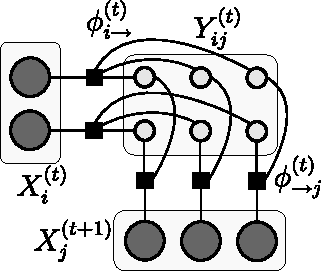
\includegraphics[width=\textwidth]{images/chaingraph/fig_crf_less_nodes.pdf}
        %\rule{\textwidth}{0.3pt}
        \caption{Factor graph representation of the conditional random field at time steps $t$ and
            $t+1$, \ie the undirected part of the chain graph. The assignment variables (smaller,
            light nodes) $Y_{ij}^{(t)}$ are conditioned on the detection variables
            $X_i^{(t)},X_i^{(t+1)}$(dark nodes).}
        \label{fig:chaingraph-crf}
    \end{subfigure}
    \hfill
    \begin{subfigure}[t]{0.48\textwidth}
        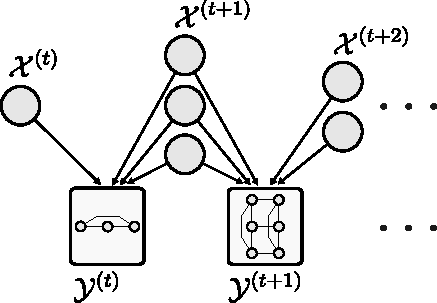
\includegraphics[width=\textwidth]{images/chaingraph/fig_chain_graph.pdf}
        %\rule{\textwidth}{0.3pt}
        \caption{In the directed part of the chain graph the conditional random fields from
            \cref{fig:chaingraph-crf} are subsumed in supernodes (boxes).}
        \label{fig:chaingraph-bn}
    \end{subfigure}
    \caption[Chain graph model]{Conditional random field representation for two consecutive time steps
        of the ``transition model'' (\subref{fig:chaingraph-crf}) and chain graph model for three
        subsequent time steps (\subref{fig:chaingraph-bn}), taken from \citet{kausler_12_discrete}.}
    \label{fig:chaingraph-model}
\end{figure}

After the recap of the chain graph tracking and the conservation tracking factor graph in
\cref{subsec:fg-chaingraph,subsec:fg-conservation}, respectively, we continue with the introduction
of cell identity reconstruction for conservation tracking~(\cref{cha:GMM}) and a new
tracking-by-assignment method, joint segmentation and tracking~(\cref{cha:joint}), which both
address the problem of undersegmentation in cell tracking.


%%% Local Variables: 
%%% mode: latex
%%% TeX-master: "../../../main"
%%% End: 



\subsection{Conservation Tracking}
\label{subsec:fg-conservation}

The chain graph tracking as described above is capable of handling an unknown number of dividing
objects, if each detection contains one cell at maximum. This means that the segmentation must
contain all cells in the data set as individual objects in order to achieve an accurate tracking
result. As a consequence, speckle noise (false positives) can be handled by chain graph tracking.
``Mergers'' however, that may occur by occlusions in 2d or due to bad imaging quality in 2d and 3d,
pose an obstacle for the chain graph tracking: When two or more cells are merged into a single
connected component due to undersegmentation, all but one of the associated tracks will get lost, as
the chain graph energies (Equations~\ref{eq:cg-cost-out} to~\ref{eq:chaingraph-cost-det}) disallow merging, \ie a
cell has more than once ancestor. From a chain graph tracking point of view, the lost tracks appear
either as disappearances or a series of false positive detections in the time steps previous to the
merging event. In a similar fashion, a demerging of a merger object cannot be handled correctly by
the chain graph tracking either. Here, the chain graph tracking would interpret the incident as a
transition from the merged object to one of its possible descendants in the next time step in
conjunction with either one or more appearances or false positive detections. Furthermore, a
demerging of two cells might be misinterpreted as a division.

Since unique detections of all cells cannot be guaranteed in dense cell populations or poor image
quality, \citet{schiegg_13_conservation} propose a method that can also handle merges. They leave
behind the assumption that a detection matches exactly one cell or is a false positive. In terms of
graphical models, this means that, in contrast to the chain graph tracking model, the random
variables are not binary, but discrete variables that carry information about how many cells they
represent (one detection variable still represents a single detection). They then apply conservation
laws that ensure ``global consistency of the solution''. This allows for detection of merged cells,
\ie detections that represent more than one cell. A more detailed description of this method is
provided in the following including an overview of the pipeline in
\cref{fig:fg-conservation-pipeline}. Reconstruction of the identities of the involved cells requires
an additional post-processing step which is our contribution and will be discussed in detail in
\cref{cha:GMM}.

\begin{figure}
    \centering
    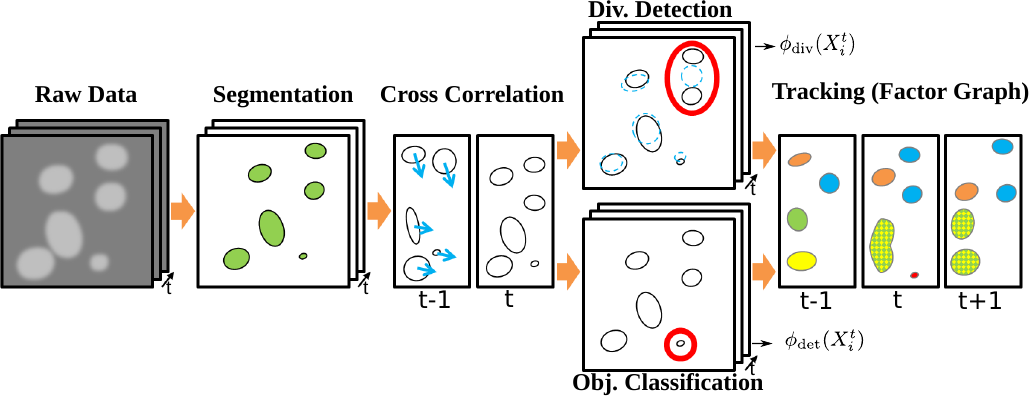
\includegraphics[width=\textwidth]{images/conservation/pipeline.png}
    %\rule{\textwidth}{0.3pt}
    \caption[Conservation tracking pipeline]{Pipeline of the conservation tracking (taken and modified
        from~\cite{schiegg_13_conservation}): First cells are detected in the segmentation
        step. Then, cross correlation is used for estimating the cell positions in subsequent
        time steps. Based on these corrected positions, the hypotheses graph is generated. Finally,
        inference on the corresponding factor graph yields a tracking result. In order to inject
        prior belief, the predictions of classifiers for divisions and the number of objects in a
        detection are taken into account in the potentials of the factor graph.} 
    \label{fig:fg-conservation-pipeline}
\end{figure}

\citet{schiegg_13_conservation} use a factor graph for modeling. To this end, they introduce
discrete multi-state random variables for detections, $X_i^t \in \{0,\dots ,m\}$,
representing connected component $i$ at time step $t$. The state of such a detection variable
determines the number of cells that are comprised in the corresponding connected
component. Additionally, transition random variables $T_{ij}^t, \in \val(T_{ij}^t)=\{0,\dots ,m\}$
represent transitions from detection $i$ at time $t$ to detection $j$ at time $t+1$. Here, the
design parameter $m$ specifies the maximum allowed number of cells per connected
component. Moreover, the transition variables can be interpreted as some ``flow'' of mass going from
detection $i$ at time $t$ to detection $j$ at time $t+1$. Then, conservation laws, hence the name
``conservation tracking'', ensure global consistency. However, appearances and disappearances are
not consistent with these conservation laws. Therefore, to allow for breaking these laws, $X_i^t$
is defined deterministically as
\begin{align}
    \label{eq:cons-det-a-v}
    X_i^t& = \max(V_i^t, A_i^t), \\
    \val(V_i^t) &= \val(A_i^t) = \{0,\dots ,m\},
\end{align}
with discrete random variables $V_i^t$ and $A_i^t$, which need not follow conservation laws, thus
making appearances and disappearances possible. Then an appearance is modeled by $V_i^t=0,
A_i^t=k>0$ (Equation~\ref{eq:fg-conservation-det-b} and a disappearance by $V_i^t=k>0, A_i^t=0$
(Equation~\ref{eq:fg-conservation-det-c}). Therefore, partial appearances or disappearances are not
possible (Equation~\ref{eq:fg-conservation-det-d}). On the contrary, $V_i^t=A_i^t$
(Equation~\ref{eq:fg-conservation-det-c}) represents a connected component, which does not appear or
disappear, \ie it has possibly multiple ancestors and descendants, with the special case of a false
positive detection $V_i^t=A_i^t=0$.
% representing the event of disapperance and
% appearance respectively. This is neccessary because an appearance means, that no mass is flowing
% into the cell, which would be a violation of the conservation law. This holds for disappearances
% analogously. Thus, the conservation law between vanishing and appearing nodes needs to be redefined:
% Both variables may be in the same state, representing a false positive detection in case of state
% zero and a transition otherwise. Moreover, either of the variables may be zero while the other is
% non-zero. This is the case when a cell disappears or appears. A partial appearance or disappearance
% is not allowed, which is enforced by disallowing configurations where vanishing and appearaing
% variable are both non-zero, but not in the same state.

Furthermore, to distinguish between a division and the demerging into two single cells, a
binary division variable $D_i^t \in \{0, 1\}$ is introduced that indicates whether a cell is dividing
into two children cells, or not.

\cref{fig:conservation-fg} shows how these random variables are brought into relation in a factor
graph. In order to pull the configuration of random variables towards a meaningful tracking
solution, the factors of this graph score configurations by assigning a high energy to states that
are unlikely to resemble a real tracking while keeping the energy of more likely, preferable
configurations low. Moreover, they disallow illegal configurations as specified above.

\begin{figure}
    \centering
    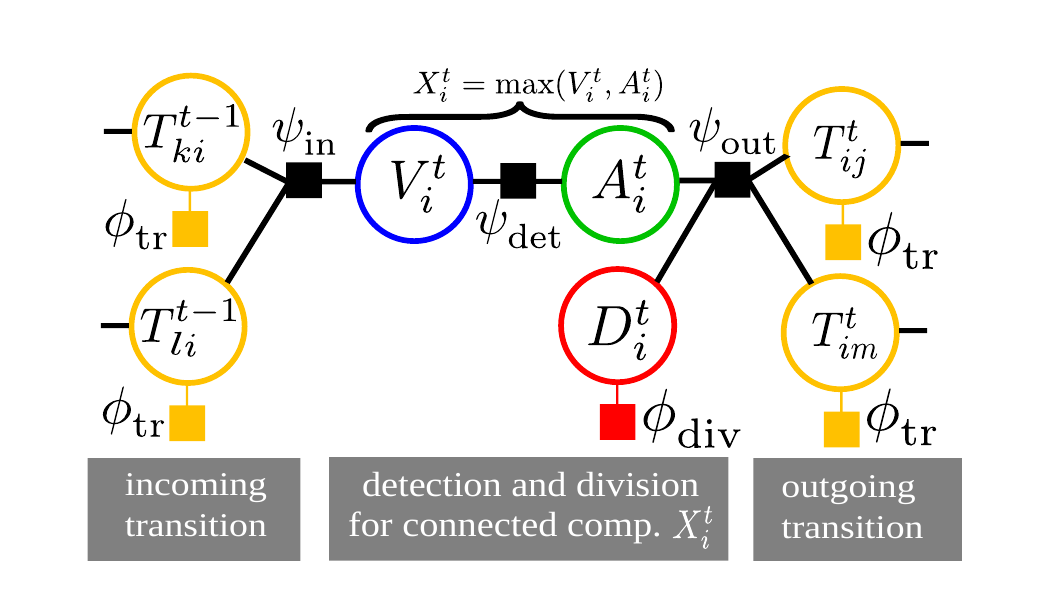
\includegraphics[width=0.6\textwidth]{images/conservation/factor_graph.png}
    %\rule{\textwidth}{0.3pt}
    \caption[Conservation tracking factor graph]{Factor graph of the conservation tracking model
        (taken from \citet{schiegg_13_conservation}): The excerpt of the factor graph shows
        variables that share potentials with a transition node, or, more precisely, with the
        vanishing node and the appearing node, that determine the state of the transition node.}
    \label{fig:conservation-fg}
\end{figure}

In the following, the factors are specified. To begin with, the \emph{detection factor}
\begin{align}
    \label{eq:fg-conservation-det}
    \psi_{\text{det}}(A_i^t,V_i^t,f_i^t) &= e^{-E_{\text{det}}(A_i^t,V_i^t,f_i^t)},
\end{align}
\begin{subnumcases}{E_{\text{det}}(A_i^t,V_i^t,f_i^t) =}
    -\log\bigl(\hat{P}(X_i^t=k|f_i^t)\bigr), &$V_i^t=A_i^t=k$ \label{eq:fg-conservation-det-a}\\
    -\log\bigl(\hat{P}(X_i^t=k|f_i^t)\bigr) + kw_{\text{app}}, &$V_i^t=0, A_i^t=k > 0$ \label{eq:fg-conservation-det-b}\\
    -\log\bigl(\hat{P}(X_i^t=k|f_i^t)\bigr) + kw_{\text{dis}}, &$V_i^t=k > 0, A_i^t=0$ \label{eq:fg-conservation-det-c}\\
    \infty, &$\text{otherwise}$ \label{eq:fg-conservation-det-d}
\end{subnumcases}
takes into account local evidence $f_i^t$, \eg size or mean, and weighs configurations according to
their probability $\hat{P}(X_i^t=k|f_i^t)$ that a connected component contains
\mbox{$k\in\{0,\hdots,m\}$} cells given $f_i^t$, as determined by a random forest
classifier~(Equations~\ref{eq:fg-conservation-det-a} to \ref{eq:fg-conservation-det-c}, \cref{cha:app-rf}). The design
parameter $m$ specifies the maximum number of cells per connected component, whereas the design
parameters $w_{\text{app}}$ and $w_{\text{dis}}$ are penalties for appearing and disappearing cells
respectively. Furthermore, $E_{\text{det}}$ forbids illegal configurations by assigning infinite
energy (Equation \ref{eq:fg-conservation-det-d}), corresponding to zero probability.

Secondly, unary factors on the transitions
\begin{align}
    \label{eq:fg-conservation-trans}
    -\log\left(\phi_{\text{tr}}(T_{ij}^t,d_{ij}^t)\right) = E_{\text{tr}}(T_{ij}^t,d_{ij}^t) = -w_{\text{tr}}
    \begin{cases}
        1-\exp\left(-\frac{d_{ij}^t}{\alpha}\right), & T_{ij}^t=0 \\
        \exp\left(-\frac{d_{ij}^t}{\alpha}\right), & T_{ij}^t > 0
    \end{cases}
\end{align}
are constructed by the squared difference between the two cells involved in the potential transition
with design parameters $\alpha$ and $w_{\text{tr}}$. As an additional feature, the authors estimate the position of a
cell in the subsequent time step and calculate the squared distance with respect to that
position. This is a penalty on the acceleration rather than on the velocity of a cell, which
represents natural behavior in a better way. More precisely, the position estimate is the result of
performing patch-wise cross correlation~\citep[Chapter~14.5]{jaehne_05_digital} on successive frames of the binary segmentation.

In a similar fashion, unary factors on the division variables
\begin{align}
    \label{eq:fg-conservation-div}
    -\log\left(\phi_{\text{div}}(D_i^t, f_i^t)\right) = &E_{\text{div}}(D_i^t, f_i^t) \\= &-w_{\text{div}}
    \begin{cases}
        \log\left(1-\hat{P}(D_i^t=1|f_i^t)\right), & D_i^t = 0 \\
        \log\left(\hat{P}(D_i^t=1|f_i^t\right), & D_i^t = 1
    \end{cases}
\end{align}
embody the probability that a cell is about to divide, provided by a random forest 
classifier trained on cell detections. Again, $f_i^t$ describes local features and $w_{\text{div}}$
is a design parameter that -- like $w_{\text{tr}}$ -- weights the division prior against the
detection prior.

Finally, the conservation laws are implemented as constraints in the outgoing factor
\begin{align}
    \label{eq:fg-conservation-out}
    \psi_{\text{out}}(A_i^t, T_{ij_1}^t,\dots ,T_{ij_n}^t) = e^{-E_{\text{out}}(A_i^t, T_{ij_1}^t,\dots ,T_{ij_n}^t)},
\end{align}
\begin{subnumcases}{\label{eq:cons-out} E_{\text{out}}(A_i^t, T_{ij_1}^t,\dots ,T_{ij_n}^t) =}
    \infty, & $\sum_{l\in \{j_1,\dots , j_n\}} T_{il}^t \ne A_i^t + D_i^t$ \label{eq:cons-out-a} \\
    \infty, & $\exists l \in \{j_1,\dots , j_n\}: T_{il}^t > A_i^t$ \label{eq:cons-out-b}\\
    \infty, & $\sum_{l\in \{j_1,\dots , j_n\}} T_{il}^t \ne 2 \text{ if } D_i^t =
    1$ \label{eq:cons-out-c} \\
    \infty, & $A_i^t \ne 1 \text{ if } D_i^t = 1$ \label{eq:cons-out-d} \\
    0, & $\text{otherwise}$ \label{eq:cons-out-e}
\end{subnumcases}
and in the incoming factor analogously. These constraints have a meaningful interpretation in the
context of mass conservation laws: Equation \ref{eq:cons-out-a} ensures conservation of mass from a
detection to the corresponding outgoing transitions. In case of a division, the additional mass is
created by the division variable (Equations \ref{eq:cons-out-a} and
\ref{eq:cons-out-b}). Furthermore, a merger cannot be a dividing object (Equation
\ref{eq:cons-out-d}). In conjunction with Equations \ref{eq:cons-out-a} and \ref{eq:cons-out-c},
this implies that a division cell must have exactly two children and that the mass involved in a
division is $2$, equally distributed on the division variable and the detection variable.

The product of all of these factors, divided by the partition function $Z$ defines the probability for
a specific configuration of all random variables:
\begin{align}
    \label{eq:fg-conservation-prob}
    P(\mathcal{A}, \mathcal{V}, \mathcal{D}, \mathcal{T}) = \frac{1}{Z}\prod_t\prod_i \Biggl(
    &\psi_{\text{det}}\left(A_i^t,V_i^t,f_i^t\right ) \phi_{\text{div}}\left(D_i^t\right)
    \prod_j\left(\phi_{\text{tr}}(T_{ij}^t)\right) \\\nonumber \times &\psi_{\text{out}}\left(A_i^t,
        T_{ij_1}^t,\hdots T_{ij_n}^t\right) \psi_{\text{in}}\left(A_i^t, T_{h_1i}^{t-1},\hdots
        T_{h_ni}^{t-1}\right) \Biggr)
\end{align}

Just as in the chain graph tracking (\cref{subsec:fg-chaingraph}), the MAP solution is inferred by
reformulating \cref{eq:fg-conservation-prob} as a Gibbs energy that is minimized in an ILP:
\begin{align}
    \argmax_{\mathcal{A}, \mathcal{V}, \mathcal{D}, \mathcal{T}}P(\mathcal{A}, \mathcal{V},
    \mathcal{D}, \mathcal{T}) & = \argmin_{\mathcal{A}, \mathcal{V}, \mathcal{D}, \mathcal{T}} E(\mathcal{A}, \mathcal{V}, \mathcal{D}, \mathcal{T}) \\
    &= \argmin_{\mathcal{A}, \mathcal{V}, \mathcal{D}, \mathcal{T}}\left(-\log P(\mathcal{A},
        \mathcal{V}, \mathcal{D}, \mathcal{T})\right).
    \label{eq:fg-conservation-map}
\end{align}

%%% Local Variables: 
%%% mode: latex
%%% TeX-master: "../../../main"
%%% End: 

%%% Local Variables: 
%%% mode: latex
%%% TeX-master: "../../main"
%%% End: 
